\chapter{Use Case: Supply Chain Management}
\section{Supply chain management}
The supply chain is the number of activities that information flow products from suppliers to customers, manage all activities related to sourcing, conversions, delivery, etc. Supply chain management, not only is beneficial in various fields such as financial, social, and world. It enhances resources, exploitation, and cyclic time from material to end-users.
Supply chain processes started within the company’s processes or distribution. We believe that supply chain management is essential for the delivery of business results\cite{Wu}.
\begin{center}
	\begin{figure}[htb!]
		\begin{minipage}{0.50\linewidth}
			
			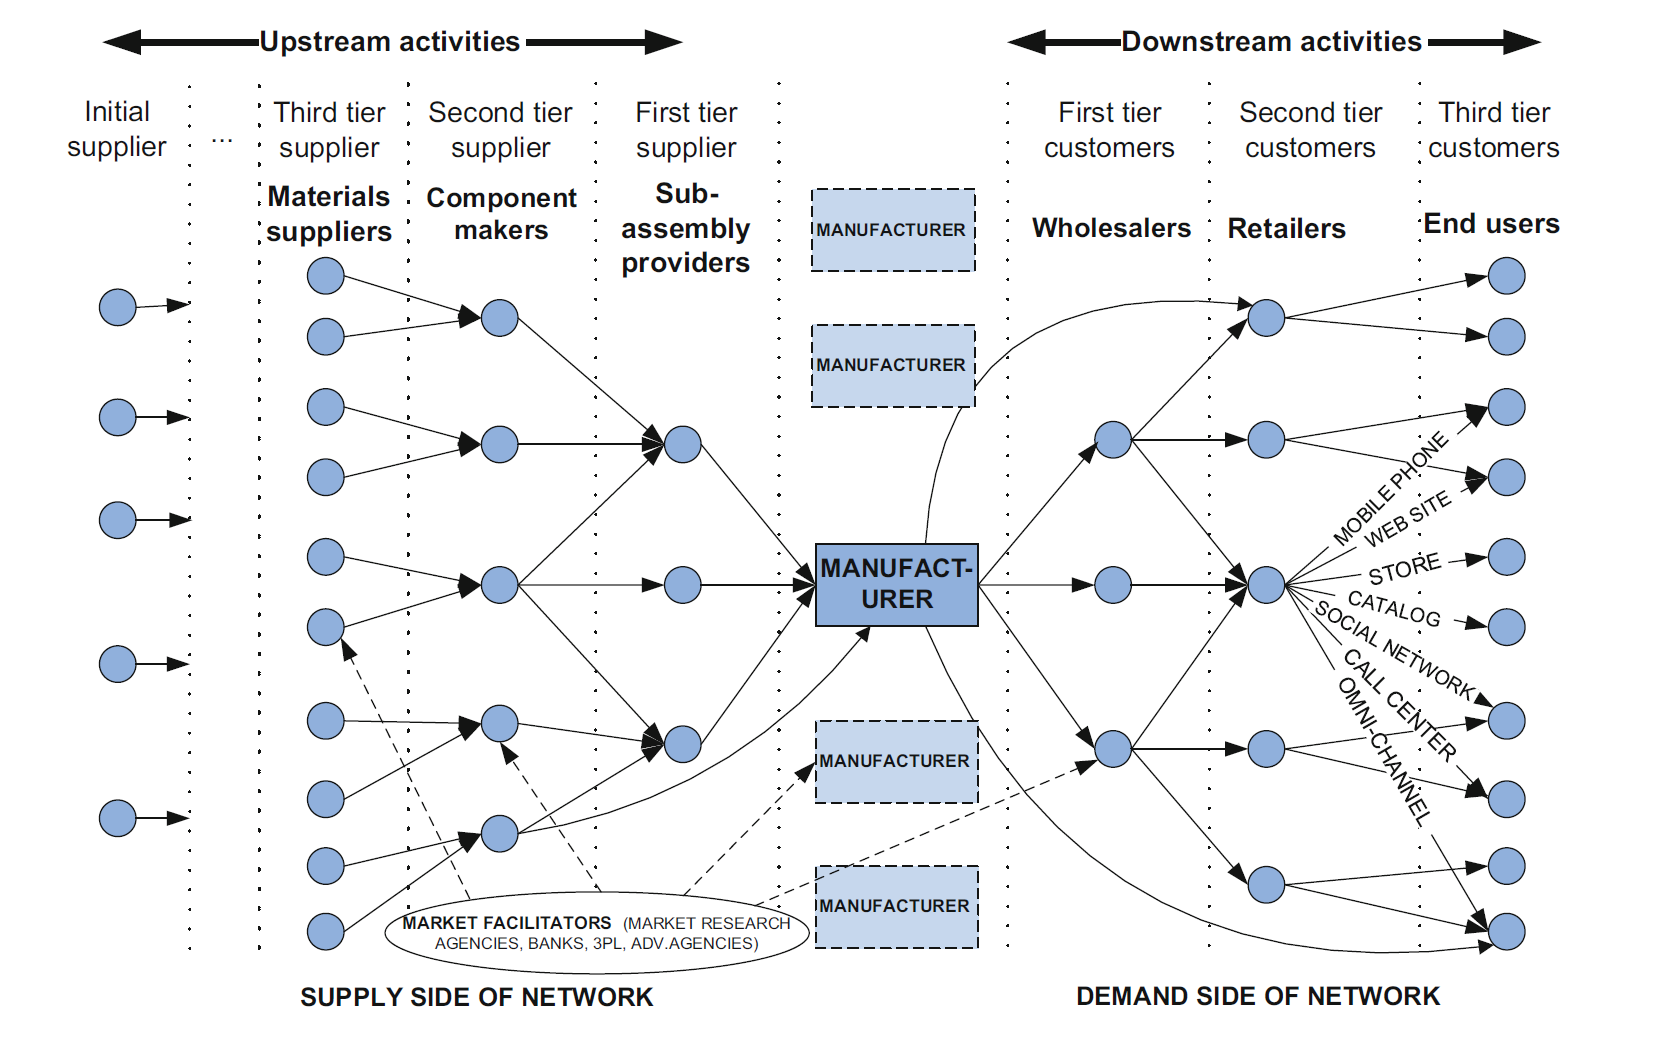
\includegraphics[width=1.85\textwidth]{images/chap03_SCM_network.png}
		\end{minipage}
		\caption{Network supply chain management\cite{Sajter}}    
	\end{figure}    
\end{center}

Supply chain management is a critical factor in global business and improvement efforts become increasingly important. Supply chain management is a great strategy that makes alignment flow of raw material, manufacturing, and distribution to the customer according to customer's demand. \\
Supply chain management is an approach that integrates the network of operating entities to the delivery system fulfilling the satisfaction of customers and protecting the competitiveness of the supply chain. 
In this regard, the Supply chain is the chain of activities and demand marketing service\cite{Kemal}. Christopher (TODO) claimed against uni-dimensional supply chain as follow:\\
\textit{"Supply chain management should be termed demand chain management to reflect the fact that the
	chain should be driven by the market, not by suppliers. Equally the 'chain' should be replaced by
	'network' since there will normally be multiple suppliers and, indeed, suppliers to suppliers as well as
	multiple customers and customers to be included in the total system."}
\section{How to improve SCM applying blockchain? }
The decentralized nature of the blockchain couple with data immunity made it appropriate for the supply chain management.
This feature provides the opportunity to fulfill the requirements of the supply chain.  
Using blockchain, from one hand store data on the supply chain, this data can not tamper easily. On the other hand, data from multiple stack holders can be integrated into the blockchain rather than stored in the individual system.
One of the critical factors in supply chain management, manufacturing management, delivery management, is data management. The type of data in the supply chain is not bounded to inventory information. Data streaming is a core process in supply chain management.
\begin{center}
	
	\begin{figure}[htb!]
		
		\begin{minipage}{0.55\linewidth}
			
			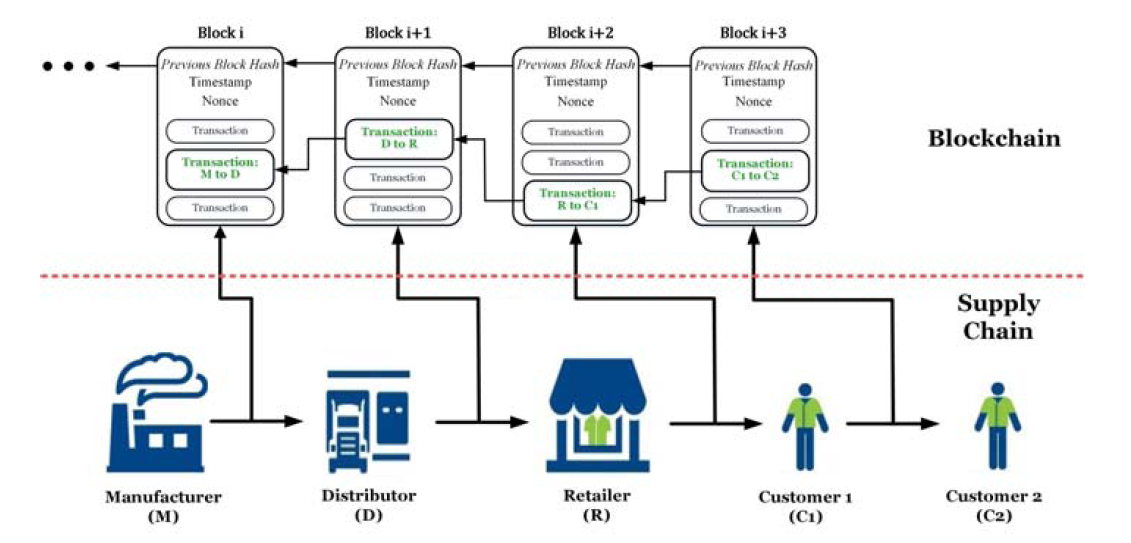
\includegraphics[width=1.85\textwidth]{images/chap03_SupplyChain_blockchain.png}
		\end{minipage}
		\caption{Supply chdain management with blockchain\cite{Nazmul}}
		
	\end{figure}
	
\end{center}
Data for SCM fed into the blockchain via information flow. In this process information flow, previous input and stack holders store data in an off-line way. Information can exchange through the postal system. One possible way is to automate information flow, but it brings some concerns such as manipulation of data veracity and violates security and time consuming of data processing. Therefore, we can improve the SCM system by sharing, information within the supply chain, protect data veracity and accelerate the data recovery.\\
But there are some issues to do this, one of them is to gather data from the external environment convert to digital information via IoT devices, smart sensors, etc. The other is to identify how to implement blockchain on SCM through various approaches. So that, they can obtain more requirement of SCM from the industry.\\
Generally, the critical property of blockchain which is decentralization cause to deal with three concerns such as Trust-less, security, and authentication. We deal with these issues in SCM by traceability, efficiency, and transparency.
Blockchain application is on an increase in payment infrastructure, cryptocurrency, and verification. In supply chain management, blockchain not only offers transparency regarding who is participating and which activities take place but also provides solutions for real-time supplier management, shipment management, identity management, etc. Blockchain is beneficial to all parties and the supply chain network. \\

\subsection{Blockchain operation in supply chain management}
The main benefits of blockchain technology applications have been concerned with how it can
provide valid information to supply chain network participants.  The need for collective activities will disappear, Through such transparent information-sharing mechanisms.
Participants can rely on transaction history to transfer assets like ether, even without needing to the third party\cite{Nina}.
Blockchain emphasized on four attributes:
1. Information synchronization: all participants have access to the same data containing a history of the transaction.\\
2. p2p network and consensus mechanism: there is no need to third authority to control transactions\\
3. Smart contact: all obligations are formalized in programming code which should be met.\\
4. Data stability: Modification must be verified just with the consensus of all participants, Not altering without collective verification\cite{Nina}. \\
Based on Four common attributes of blockchain
summarized in table follow:\\
\begin{table}[h!]
	\begin{center}
		\begin{adjustwidth}{-1cm}{}
			
			\begin{tabular} { c | c | c | c | c | c }
				
				\tiny \textbf{Context} &\tiny \textbf{Logistic}\cite{Tijan} & \tiny \textbf{HealthCare} & \tiny \textbf{Banking}\cite{Guo} & \tiny \textbf{Engineering}\cite{Kontantinos} & \tiny \textbf{Green SCM}\cite{Sarkis} \\
				\hline
				\tiny \makecell{Information\\ synchronization} & \tiny \makecell{digital version\\ of a ledger to\\ decentralized\\ system participants\\ to follow data} & \tiny \makecell {Allow copies of\\ patient's record\\ to update with \\participants records} & \tiny \makecell{Remove link of \\third party financial\\ institution\\ in distribution\\ of goods} & \tiny \makecell{participants interact\\ with blockchain via\\ private and\\ public key} & \tiny \makecell{all participants\\ have same copy\\ of ledger which\\ is updatable\\ by new modification \\in blockchain}\\ 
				\hline 
				\tiny P2P network   & \tiny \makecell{participants share \\transaction with\\ blockchain and\\ copy of ledger}& \tiny \makecell{Participants have \\copy of whole\\ blockchain to\\ ensure that \\date is authenticated} & \tiny \makecell{Helping system\\
					participants control \\big data and
					\\constructing ownership} & \tiny \makecell{transaction broadcast \\into blockchain via \\user's node} & \tiny \makecell{Participants can\\ follow record of\\ transaction, thus\\ can track performance \\of transportation}\\ 
				\hline
				\tiny Smart contract   & \tiny \makecell{legal provision\\ are formalized\\ into code and\\ verified through a \\network of peers } & \tiny \makecell{records stored on\\ blockchain } & \tiny \makecell{ensure that\\ payment is\\ done automatically\\ after reaching\\ result and\\ reduce manual\\ risk} & \tiny \makecell{script storing\\ in blockchain\\ is similar to stored\\ procedure in\\ relational database\\ management system} & \tiny \makecell{Automatic payment\\ is done, when\\ regulations are\\ met or value\\ added to products}\\ 
				\hline
				\tiny Data stability   & \tiny \makecell{ transaction are\\ approved by\\ consensus of all\\ participants, it \\stores in block } & \tiny \makecell{Create indecomposable \\databases for medical \\records and tracing\\
					pharmaceuticals\\ through manufacturing\\
					and distribution} & \tiny \makecell{after entering\\ information into\\ system, can not\\ be altered, thus preventing\\ from subsequent\\ fraud} & \tiny \makecell{transaction will\\ be verified\\ through hash\\ of previous block\\ in blockchain} & \tiny \makecell{Tracing the waste, \\distribution\\ responsibility to\\ system participants \\for cleanup\\ cost}
				
				
				
			\end{tabular}
		\end{adjustwidth}
		\caption {Summary of blockchain characteristics in various contexts supply chain management.}
	\end{center}
\end{table}

\subsection{Analysis of supply chain ontology models}

This section reports on the analysis using the comparison
framework. The analysis presented here provides insights into
the gaps in existing supply chain ontology research. The table lists these ontologies shows the
values for the criteria application, scope, KR paradigm, language, and methodology approach.\\
\textit{Scope} concerns with the field of industry which used in ontology.\\
\textit{Language} is the type of language that is used in ontology.\\
\textit{Application} is concerned with the type of problem-solving task for which the ontology is to be used.
These tasks span a wide range of applications in the supply chain.\\
\textit{Key concept} is about main concept used in ontology.\\
\textit{Purpose} concern to use ontology using in supply chain\cite{Tonci}.\\ 


\begin{landscape}
	
	\begin{table}[ht!]
		\begin{center}
			\begin{adjustwidth}{}{}
				\begin{tabular}{ c | c | c | c | c | c | c | c  } 
					
					\tiny \textbf{\makecell{Supply\\ chain\\ Ontology\\ model}} & \tiny \textbf{\makecell[l]{KR \\paradigm}} & \tiny \textbf{Language} & \tiny \textbf{Scope} & \tiny \textbf{Purpose} & \tiny \textbf{Key concept} & \tiny \textbf{\makecell[l]{Methodically\\ approach}} & \tiny \textbf{\makecell[l]{Application}}\\
					
					\hline  
					
					\tiny \textit{\makecell{Model by\\ Sousa at al.\cite{Sousa}}} & \tiny \makecell[l]{Algebra \\of sets} & \tiny UML & \tiny \makecell{Business\\ network} & \tiny \makecell[l]{Improve manufacturing \\performance of virtual \\enterprise by bridging \\gap between planing \\level and control level\\, integrating incoherent \\manufacturing systems}& \tiny \makecell[l]{plan, unit, product,\\ organization,\\ order, resource,\\ customer, activity.}&  \tiny \makecell[l]{Combination of generic\\ techno-organizational\\ requirement and synthesis\\ of ontology} & \tiny \makecell[l]{ Production and\\ operation planning \\virtual enterprise of\\ and control \\semiconductor industry}\\
					
					\hline
					
					\tiny \textit{\makecell{TOVE\\ ontology\cite{Kim}}} & \tiny DL  & \tiny \makecell{XML} & \tiny \makecell{internal \\ supply\\ chain} &\tiny \makecell[l]{Develop enterprise\\ model which will\\ have ability to deduce\\ answer queries in\\ industrial environment}  & \tiny \makecell[l]{agents, roles,\\ positions, activity,\\ resource, commitment,\\ communication,\\ authority} & \tiny \makecell[l]{Ontology developed\\ and comply to\\ pose competence\\ questions at \\the beginning} & \tiny \makecell[l]{Using TOVE \\model to analyze\\ enterprise\\ ontology}\\
					
					\hline
					
					\tiny \textit{\makecell{IDEON\\ ontology\cite{Madni}}} & \tiny \makecell[l]{Algebra \\of sets} & \tiny UML & \tiny \makecell[l]{inter-business \\network} & \tiny \makecell[l]{provides a common\\ foundation for designing,\\managing,
						and controlling\\ collaborative, distributed\\ enterprises} & \tiny \makecell[l]{process, organization, \\resource, enterprise, \\product} & \tiny \makecell[l]{there is no formal\\    evaluation, however\\ the ontology was\\ assessed based on\\ its actual uses\\ against the purposes.} & \tiny \makecell[l]{support multiple enter-\\prise
						applications: Crisis\\ Action Planning and\\ Integrated Product-Process\\ Development which enabled\\ systems engineering.} \\     
					
					\hline
					
					\tiny \textit{\makecell{Model by \\Ye at al.\cite{Ye}}} & \tiny DL & \tiny \makecell[l]{OWL, SWRL} & \tiny \makecell[l]{inter-business\\ network} & \tiny \makecell[l]{serve as an interlingua\\ to enable
						information \\integration across interacting\\ applications and semantic\\ integration of heterogeneous \\system in supply chain} & \tiny \makecell[l]{structure, activity,\\ performance, purpose, \\role, party, transfer} & \tiny \makecell[l]{SCOR provides a basis\\ for
						describing the \\knowledge of supply chain\\ performance; The same\\ methodology for the\\ development of EO\\ was used} & \tiny \makecell[l]{application integration\\ framework based\\ on developed ontology\\ is used to solve\\ problem of information\\ integration}\\
					
					\hline
					
					\tiny \textit{\makecell{EAGLET\\ ontology\cite{Geerts}}} & \tiny \makecell[l]{} &\tiny UML & \tiny \makecell[l]{supply chain\\ of thing}& \tiny \makecell[l]{facilitate the visibility\\ and inter-operability of\\ things along the \\supply chain.} & \tiny \makecell[l]{Event,
						agent,\\ location, equipment,\\Thing}& \tiny \makecell[l]{Hybrid:inspiration, \\synthesis and \\ compliance of\\ this ontology with\\ real-world practices\\ is much higher.} & \tiny \makecell[l]{1. extend formalization\\ beyond current knowledge\\ 2. address more supply\\ chain practice; \\3. used as an instantiation\\ pattern; 4. focus\\ on fixed asset and\\ agent visibility} \\
					
					\hline
					
					\tiny \textit{\makecell{MSE ontology\cite{Lin}}} & \tiny DL & \tiny RDF, OWL & \tiny \makecell[l]{inter-business\\ network} & \tiny \makecell[l]{provide semantic and\\ syntactic interoprability\\ service to enable\\ understanding of basic\\ manufacturing terms \\between different \\manufacturing system\\ engineering enterprise \\applications} & \tiny \makecell[l]{product, enterprise,\\ project, process,\\ resource, strategy, flow} & \tiny \makecell[l]{built on the\\ experiences and\\ knowledge of \\published\\ manufacturing\\ system information\\ models.}        
					& \tiny \makecell[l]{There are some \\application area\\ thereby companies\\ enter into tempoSEMrary\\ inter-enterprise\\ collaboration for\\ exchanging information} \\
					
					\hline
					
					\tiny \textit{\makecell{Enterprise \\ontology\cite{Uschold}}} & \tiny \makecell[l]{} & & \tiny \makecell[l]{not \\applicable}& \tiny \makecell[l]{facilitate enterprise\\ design and
						analysis by\\ supporting\\ communications among \\human} & \tiny \makecell[l]{person, activity,\\ plan, resource,\\ marketing,\\ organization, \\purpose, strategy} & \tiny \makecell[l]{inspiration and \\synthesis;\\
						ontology was assessed \\based on its uses\\ against the original\\ purposes.} & \tiny \makecell[l]{improve method with\\ a framework for \\integrating method and\\ tools which are\\ appropriate to enterprise\\ modeling and management \\of changes }
				\end{tabular}
				
			\end{adjustwidth}
		\end{center}
		\caption{Different supply chain ontology models}
	\end{table}
	
	
\end{landscape}

\section{How smart contract improve supply chain}
Before the era of smart manufacturing, supply chain management is and log process called a black box, in terms of input-output mechanism. This black box consists of multiple mini processes related to the product, services, customer, etc. Many possible by emerging new technology like smart sensor and IoT devices, This long process is made more cost-effective, transparent. Meanwhile, a collaboration between supply chain structures bring strategic benefit to involve all parties.\\
Using some new technology in supply chain management such as smart contract, IoT devices and a consensus mechanism in blockchain make this system more cost-efficient, efficient, and secure at the same time. A smart contract can be implemented throughout the life-cycle of the supply chain process of raw-material to end-users. For instances, a smart contract can be used in terms of demands of product personalization, utilization, and services, subsequently, automated payment machines that are connected to IoT can cooperate using the smart contract in terms of the requirement that must be met before going to next machine.\\
Besides, Based on the blockchain with logic rules, a smart contract can be used to control quality and cont management between company and Original Equipment Manufacturer(OEM). Also, manufacture can use smart contract with the authorized provider in terms of how the product should be repaired or updated and son on.\\ (blockchain-based trust mechanism IOT)
Furthermore, a Smart contract can simplicity the performance of the supply chain and improve transparency across the supply chain. Using IoT devices to track the locations of goods. A smart contract can be helpful in this case determining the provenance of goods. This is an important part of all industries special in food industries. recently, some big companies start using smart contract to trace the device racing the goods, including meat, foods, containers, and even diamond\cite{Adam}.

\section{How smart contract works?}

To understand how smart contract works?, the first we should know how Etheruem operates and how smart contract comes into play?
could any The main term of Etheruem is an account, any time that there is exchange information between accounts, it captures in the blockchain.\\
There are two accounts in Ethereum: One is externally owned account that controlled by a private key, the other is a contract account which is activated by EOA and controlled by internal code.\\
To create a smart contract, the participant should identify an opportunity to agree to other parties. This could any values such as good and service. Then they must set terms and conditions that have to b met. This could be triggered by participants or external events. All agreement will be written in code as a smart contract which can be deployed in the blockchain were executed by first initiating contract.\\
To initiate a smart contract, the participant fulfills the transaction with a contract account encrypted by the private key and transmitted to other nodes in the blockchain. The other participant verifies the transaction if it is triggered by a valid participant. After all, the transaction is added to the blockchain after obtaining consensus by the majority.\\
Then, a smart contract will be executed and recorded, finally, all nodes are updated in the network. But already mentioned, the outcome not altered and just states of blockchain will change. Note that, every initiator has to pay for the transaction fee to create changes in the state of the Ethereum platform. The smart contract used in Ethereum to store information on blockchain securely\cite{Angwei}.\\

\section{Addressing supply chain using smart contract: }
Using a blockchain guide to solve cooperation challenges in SCM. Blockchain improves the transparency and verification in supply chain and smart contract handle the exchanges between many participants and nodes in the blockchain.\\
A smart contract can handle improve this issue three factors: Tractability, efficiency, and transparency. \\
\begin{itemize}
	\item \textit{Transparency:} Supply chain improves traceability in the supply chain by storing provenance of goods on blockchain. this will ensure the manufacture were goods, the raw material are coming from valid sources and customer have more confident that purchase legal products.\\ 
	Another usage of smart contracts in the supply chain. Also, transparent authentication across the supply chain. Participants can verify easily each other using certification stored in the blockchain in digital form. All together, allow the supply chain manager to have a correct decision when selecting a supplier to work with.\\
	\item \textit{Traceability:} Smart contract helps the supply chain in terms of traceability in a way that it can easily trace the inventory at every long way From raw-material to end-user delivery. The product can be traced using the serial number, tags or smart sensors.\\
	With the growth of IoT, the device can be connected. the smart sensor provides some information such as location, environment, and quality of the product. Another problem in the supply chain process is that the goods will be depreciated when arriving in users due to delays. Smart contract attributes ca mitigate delay, keeps the supply chain agile to be full- equipped to cope with the product delivery distribution such as natural catastrophe, etc. \\
	As already mentioned, one of the main usage of the smart contract is tracing the inventory in the supply chain and facilitated the supply chain system to track the products.\\
	\item \textit{Efficiency:}  Smart contract can also improve the efficiency of the supply chain in a way that using the self-executed attribute of smart contracts to help supply chain to eliminate the paperwork method and just executed smart contract only any time that obligations are met. Anther thins that using the smart contract as code enhances the cost-efficiency. because it eliminates numerous documents and paperwork required. it helps to reduce costs and amount of effort undertaken\cite{Angwei}.\\ 
\end{itemize}

\section{Concept of supply chain }
To understand the supply chain process, the author analyzed the stack holders. In figure 3.1 indicate different exchanges between stack holders that could be information, goods, or products. This is necessary to understand the requirements of stack holders to manage the supply chain process.
\\
\begin{center}
	
	\begin{figure}[htb!]
		
		\begin{minipage}{0.75\linewidth}
			
			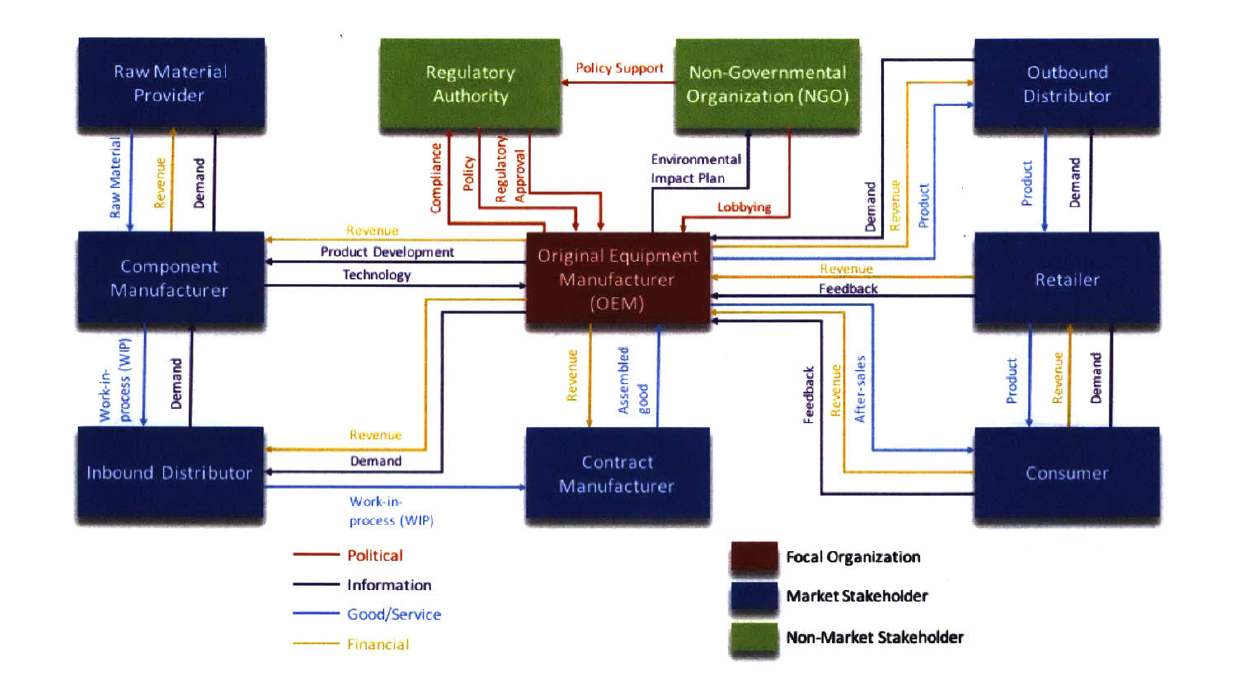
\includegraphics[width=1.45\textwidth]{images/chap03_stackholders.png}
		\end{minipage}
		\caption{Stack holders network for a generic supply chain}
		
	\end{figure}
	
\end{center}

\begin{itemize}
	\item \textbf{OEM: } Original Equipment Manufacture has a key role among all stack holders. OEM has multiple tasks such as forecasting demands of customers, inventory management, control flow, and product development, and marketing. The main goal of OEM is to develop a product, distribute them, observe satisfaction of the customer by fulfilling their demands.\\
	\item Raw-material: it is the first phase in the supply chain where it's responsible for providing the raw material for manufacture providing a high quality of raw material.
	\item Component Manufacture: raw material is used by component manufacturers to produce components with high quality and earn revenue and trust of OEM in return.
	\item Inbound Distributor: Obtain components from manufacture to distribute it to contract manufacturing assembly.
	\item Contract Manufacture: the OEM can choose to outsource final assembly to contract manufacturers to build the product.\\ 
	\item Outband Distributor: it receives the final product from OEM and distributes it to retailers for sale.
	\item Retailer: It is responsible for the sale of the product to the customer. Maximize the sale of the product and enhance the quality of the products.
	\item Customer: It is the end of the supply chain process and is the main source of demand.
	\item Authority: This is nonmarket stakeholders and has the main role in this process to ensure that products meet requirements and minimize danger.
	\item Non-Governmental Organization(NGO): It is a non-market stakeholder that has an impact on the product. Their goal is to public awareness of issues and increases their popularity\cite{Angwei}.  
	
\end{itemize}
\section{Challenges encountered in Supply chain}
As the supply chain is a long and complex process. There are some challenges which segregated into two types:\\
\begin{itemize}
	
	\item \textbf{Planning stage:}\\
	It deals with forecasting the customer demands from one hand and inventory management on the other hand. 
	\textit{Demand prediction} is the main challenge in the supply chain. The supply chain develops some models to deal with this issue. As the demand of customers changes over time.
	The supply chain builds up some models and analysis methods to predict demand using data and other characteristics.  \\
	\textit{Inventory management}, the supply chain tries to keep balancing between supplier and customer. If the supply chain is too low, the client and customer relationship will be affected negatively. If the supply is too high, that will have much inventory and it costs lower price. Apart from all, the most important thing in this process is time managing to minimize delay and delivery time to customers. The supply chain builds some models to fill the inventory to maximize profit and minimize costs.
	
	\item \textbf{Coordination stage}:
	Due to multiple stockholders in the supply chain, it exists information inconsistency. Lack of information poses some challenges in the supply chain that we referred to some of them. It affected the product traceability negatively. Lack of real-time information to track the product, it is difficult to update demand prediction and consequently destroys the trust between stack holders. One suspects information is being held by others and so on.\\ 
	Also, product quality and information sharing hold the business structure together, which allows the supply chain to improve coordination and product quality, manage the risk or distribution due to natural catastrophe\cite{Angwei}. 
\end{itemize}
\section{How to improve challenges using smart contract?}
Supply chain used smart contract to deal with three concerns:\\
1- Provenance of goods\\
2- Good traceability\\
3- Using an open database to build trust between stack holders\\
To determine \textbf{provenance}, Supplier A(main supply chain) records the detail of raw material by the usage of the smart sensor the location of materials and time of shipping can be stored into the blockchain which will be available to all parties.\\

Using the provenance the source of the product will be verified for all parties. To \textbf{tracking} the product, all parties should record all detail of shipment in the blockchain. Whenever a good received on the specific location, the contract will be triggered by the shipping party. The task of OEM is to determine the time and location of shipping .\\
\begin{center}
	
	\begin{figure}[htb!]
		
		\begin{minipage}{0.55\linewidth}
			\centering
			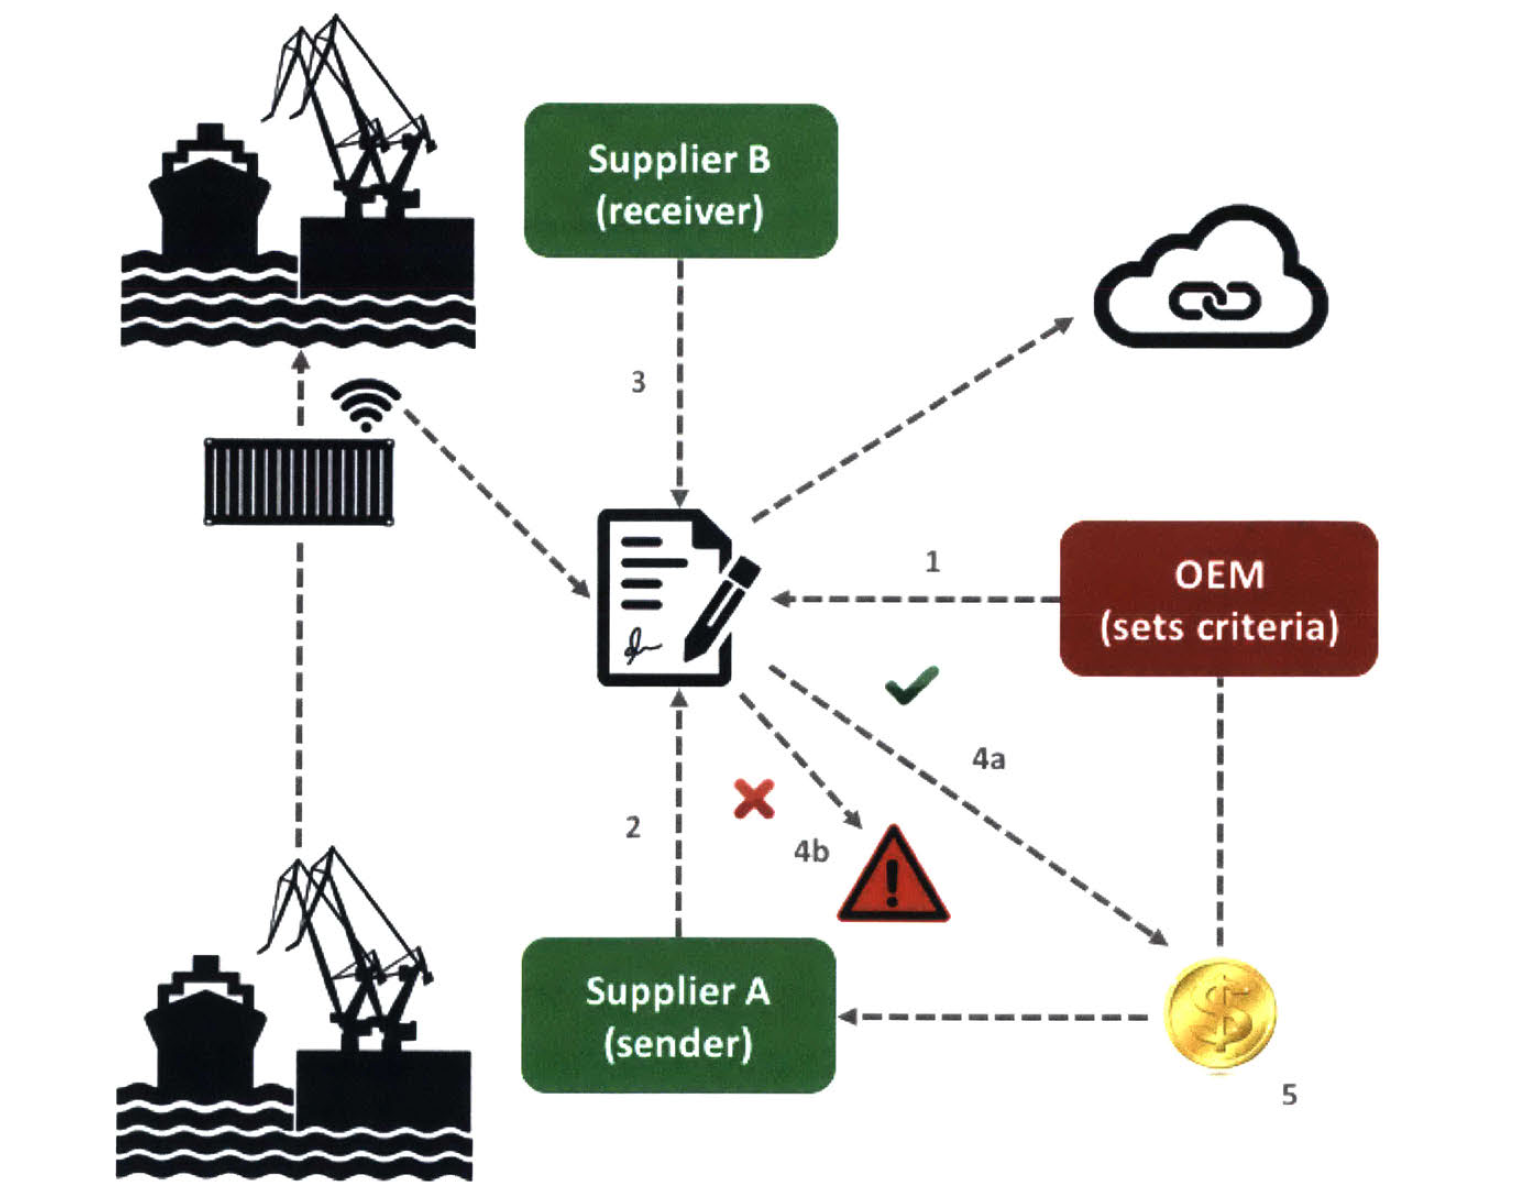
\includegraphics[width=1.65\textwidth]{images/chap03_tracking_SCM.png}
		\end{minipage}
		\caption{Using smart contract to track the goods in supply chain management}
		
	\end{figure}
	
\end{center}

Supplier A, send a shipment to Supplier B and record on the blockchain. Supplier B also records on the blockchain by receiving the shipment. The smart contract then checks whether all predetermined obligations are met.
Afterward,  payment will carry out otherwise, an alert is triggered to parties to eliminate problems.  Automate tracking helps to simplify the supply chain process and update states. That's why the supply chain will be more agile to un-predicted situations.\\ 
As already said, the supply chain is\textbf{open database} where all parties can store the detail of information in the blockchain. By every shipment, the reputation or credit of parties will increase which would be included a smart contract for tracking goods. When smart contracts call a contract for a transaction,  score (credit) also be accessible. The open database helps smart contracts for more transparency\cite{Angwei}.

\subsection{proof of concept development }
The tracking contract lets the parties trace the shipment of goods and execute the payment automatically once the shipment is completed and predetermined conditions are met. In smart contract event used to display a message when the transaction is executed. Smart contract here consists of some functions as follows:\\
\textbf{getBalance} it allows parties to check the balance of an account by inserting public address.\\
\textbf{arrived}: is an alert function which shows the number of goods and address, whenever good arrive at the destination.
\textbf{arriveGood} it allows receiver records all detail of goods on blockchain once goods are received. The receiver checks whether the items are received matches with those that are shipped. if they match, an event is triggered that the item has been received successfully otherwise it fails.\\
\textbf{sendGood} sender records all information about goods as soon as goods depart. A mapping is used to map the tracking the goods like address quantity and item. Also, goods are traced with a real-time location using sensors and other information such as time and address recorded into blockchain. An event will be triggered as the item has been shipped.\\
\textbf{checkSuccess} This allows any of the parties to check the number of a successful shipment.
\textbf{getDetails}: Gets all the details for the package contract in a call and returns all of the public members of the contract. 

\subsection{Smart contract Validation}
Remix IDE is a browser-based compiler that enables users to compile contract with solidity code. It simulates EVM  to execute the smart contract and debug it.  As executing the smart contract on Ethereum costs some
ether, Remix provides an environment to compile and debug it without any transaction fee. \textit{Figure 3.5} Figure 3.5 represents a screenshot of the Remix IDE, where the cost of executing a
contract (goodTracking.sol), transaction (sendGood)and it's output are represented: 


\begin{center}
	
	\begin{figure}[htb!]
		
		\begin{minipage}{0.55\linewidth}
			\centering
			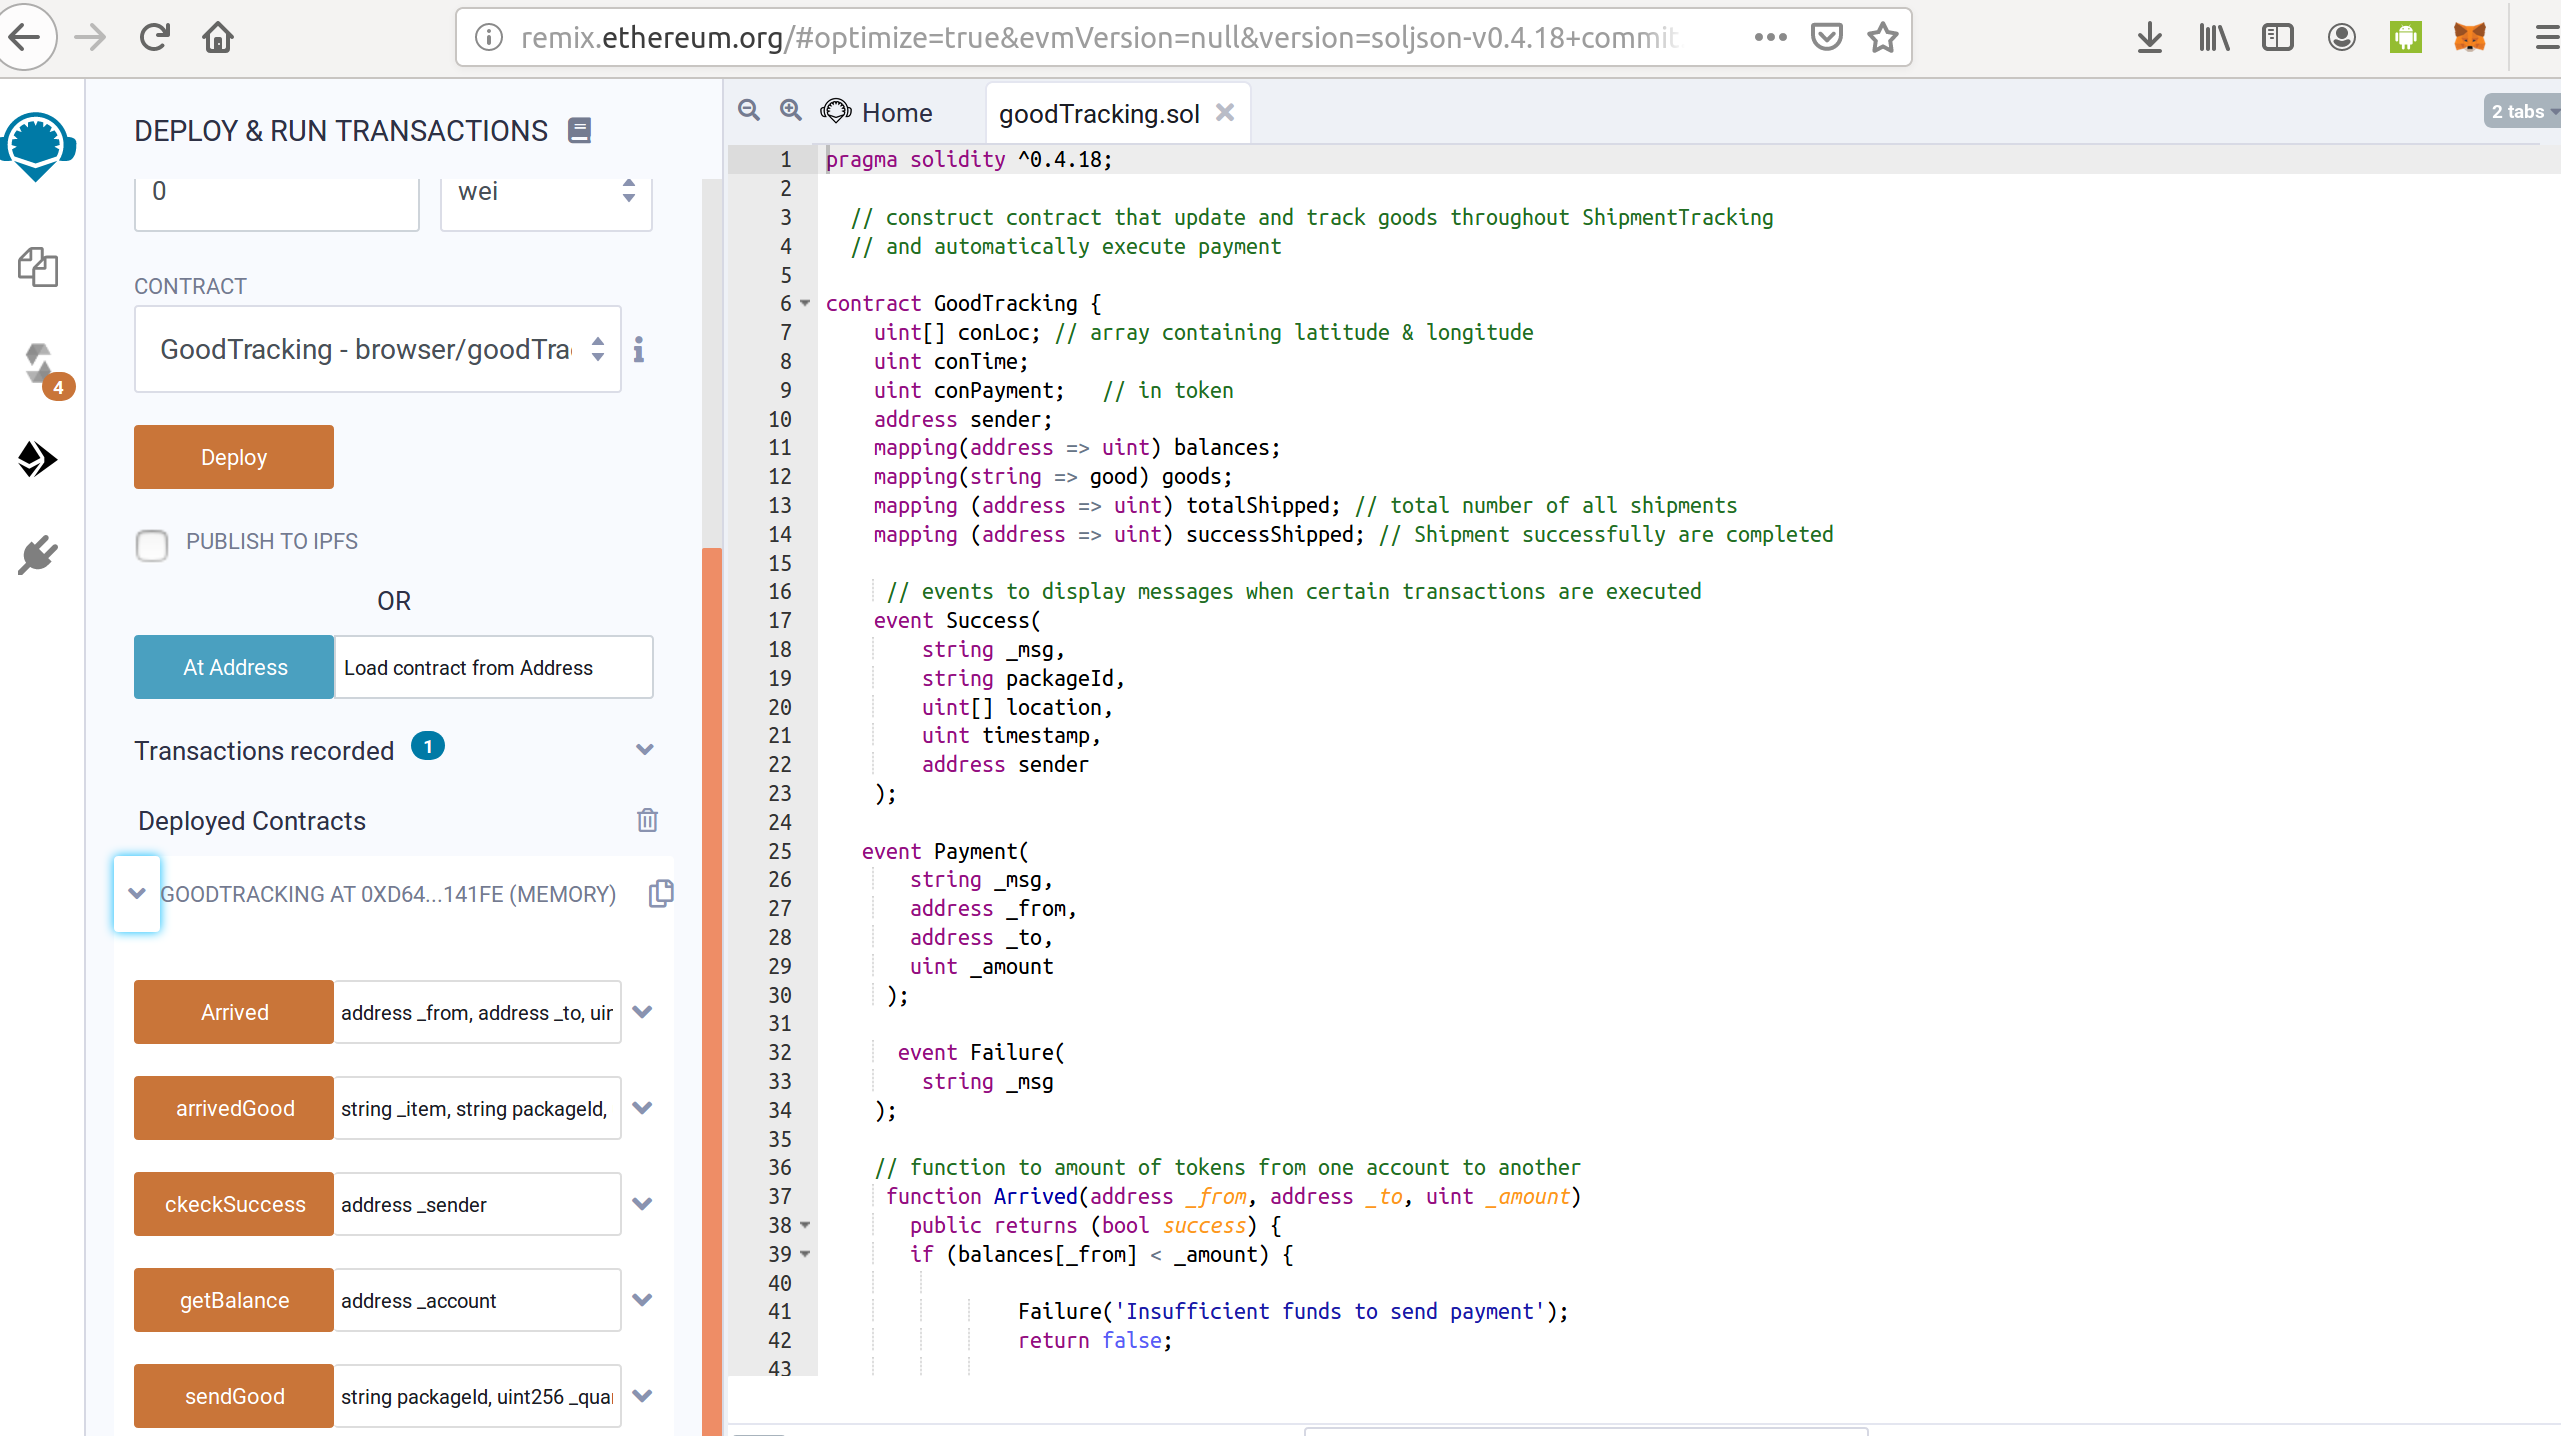
\includegraphics[width=1.55\textwidth]{images/chap03_remix.png}
		\end{minipage}
		\caption{Remix IDE to deploy shipment tracking smart contract}
		
	\end{figure}
	
\end{center}

To validate the smart contract, the contract deployed with some tokens to the administrator. Admin sets contract to ship good from supplier $A$ to supplier $B$. When supplier $A$ send good and record detail on the blockchain. When supplier $B$ receives good, records detail also on the blockchain. When the shipping quantity is not matched, an alert is triggered and fail smart contract to deploy.

\begin{center}
	
	\begin{figure}[htb!]
		
		\begin{minipage}{0.55\linewidth}
			\centering
			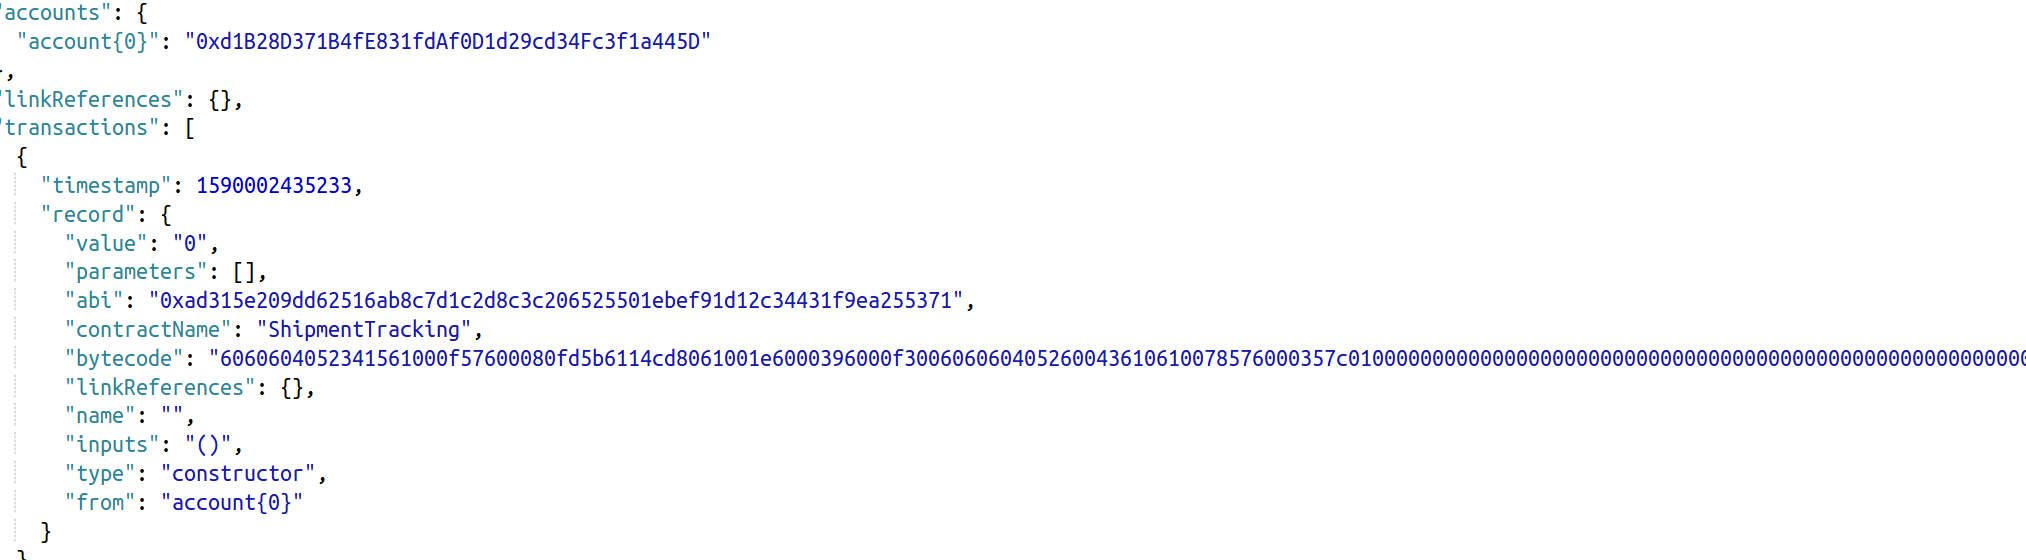
\includegraphics[width=1.55\textwidth]{images/chap03_ABI.png}
		\end{minipage}
		\caption{Recorded transactions after deploying smart contract}
		
	\end{figure}
	
\end{center}


\section{Semantic Blockchain development Implementation}
There is limited work integrating semantic in blockchain, especially smart contracts. There exists only some work on Ethereum ontology which describes blockchain concepts using RDF schema and OWL. This analysis used Ethereum ontology which describes basic semantic concepts related to specific schemas such as transactions or blocks. I used specific concepts to the transaction that I used in this study.\\
EthOn represents different models such as block, account, smart contract concepts, instances, and relation.
Ethereum ontology covers concepts and relations between objects. As my goal is to extend ontology to support my favorite schema based on a dataset by mapping to EthOn blocks or transactions model.\\
EthOn describe concepts, block, a transaction in a machine-readable format that can facilitate reasoning which can be supported our semantic web service description
Some possible ways to semantify blockchain:\\
\textbf{Step 1.} Create schema of blockchain or transaction, mapping of these data to RDF make using of vocabularies and remote procedure calls.\\
\textbf{Step 2.} Using blockchain data storage as input that will be mapped based on these data.\\
\textbf{Step 3.} Create properties of all blocks or transactions..\\
\textbf{Step 4.} Mapping all block properties to block dataset and generates an output of all inputs.\\
\textbf{Step 5.} Copy output in turtle file where related prefixes are defined.\\
\textbf{Step 6.} Generate output based on SPARQL query and data produced on the previous step.\\

\subsection{Proof of concept}
\textit{Dataset}: The main part of our analysis is the dataset which can be exported by some block explorer such etherscan that is used in this research. Dataset will feed into our Ethereum ontology mapping which each attributes map to responding values of the dataset.\\
\textit{Etherscan} is block explorer which allows us to search Ethereum blockchain for the transaction, contract, blocks, addresses, price, and other activities takes place on Ethereum.\\
\textit{Template} is in the form of RDF triple based on subject predict object that contains the prefix of concepts, Ethereum ontology concepts, our schema with the type of concepts in ethOn and instances such as integer, hex binary, boolean and string.\\

\begin{lstlisting}
ibb:{{tx_block_number}} ethon:containsTx tx:{{tx_hash}} .
tx:{{tx_hash}}  ethon:number 
"{{tx_block_number}}"^^xsd:hexBinary .
tx:{{tx_hash}} ethon:blockCreationTime "{{tx_block_timestamp}}"^^xsd:dateTime .    
tx:{{tx_hash}}  ethon:from "{{tx_from}}
"^^xsd:hexBinary .    
tx:{{tx_hash}}  ethon:to "{{tx_to}}
"^^xsd:hexBinary .    
tx:{{tx_hash}}  ethon:address "{{tx_address}}"^^xsd:hexBinary  .    
tx:{{tx_hash}}  ethon:txGasPrice  "{{tx_gas_price}}"^^xsd:integer .    
tx:{{tx_hash}}  ethon:txGasUsed  "{{tx_gas_used}}"^^xsd:integer .    
tx:{{tx_hash}}  ethon:ValueTx  "{{tx_value}}"^^xsd:integer .
\end{lstlisting}

\textit{Mapping function} is used to triple and map all the properties of the dataset, our schema and Ethereum ontology concept to each other.\\

\begin{lstlisting}
function tripleize (data, template){
let properties = {
tx_hash: (data[0][0]),
tx_block_number: data[0][1],
tx_block_header: data[0][2],
tx_block_timestamp: data[0][3],
tx_from: data[0][4],
tx_to: data[0][5],
tx_address: data[0][6],
tx_gas_used: data[0][8],
tx_value: data[0][9],
};
\end{lstlisting}

\textit{Tripleize Application} used to feed relative dataset to Ethereum ontology concepts and our schema and integrated data.(See appendix for more detail)
\textit{Header} of output formed the prefix of out concepts.
\begin{lstlisting}
@prefix ethon: <http://ethon.consensys.net/> .
@prefix ibb: <http://ethon.consensys.net/Block#> .
@prefix ibu: <http://ethon.consensys.net/Uncle#> .
@prefix ibs: <http://ethon.consensys.net/State#> .
@prefix tx: <http://ethon.consensys.net/Tx#> .
@prefix xsd: <http://www.w3.org/2001/XMLSchema#> .
\end{lstlisting}
\textit{Sparql} query is an RDF query languages that is semantic query language for dataset- enable to present and manipulate data  stored in Resource Description framework.(see appendix for full source code). \\

\begin{lstlisting}
PREFIX : <http://ethon.consensys.net/>
PREFIX dc: <http://purl.org/dc/elements/1.1/>
PREFIX ns: <http://www.w3.org/2003/06/sw-vocab-status/ns#>
PREFIX v0: <http://ethon.consensys.net/v0/>
PREFIX owl: <http://www.w3.org/2002/07/owl#>
PREFIX rdf: <http://www.w3.org/1999/02/22-rdf-syntax-ns#>
PREFIX xml: <http://www.w3.org/XML/1998/namespace>
PREFIX xsd: <http://www.w3.org/2001/XMLSchema#>
PREFIX rdfs: <http://www.w3.org/2000/01/rdf-schema#>

SELECT   ?class ?p ?o
WHERE
{
?class ?p  ?o

}

\end{lstlisting}

\begin{center}
	
	\begin{figure}[htb!]
		
		\begin{minipage}{0.55\linewidth}
			\centering
			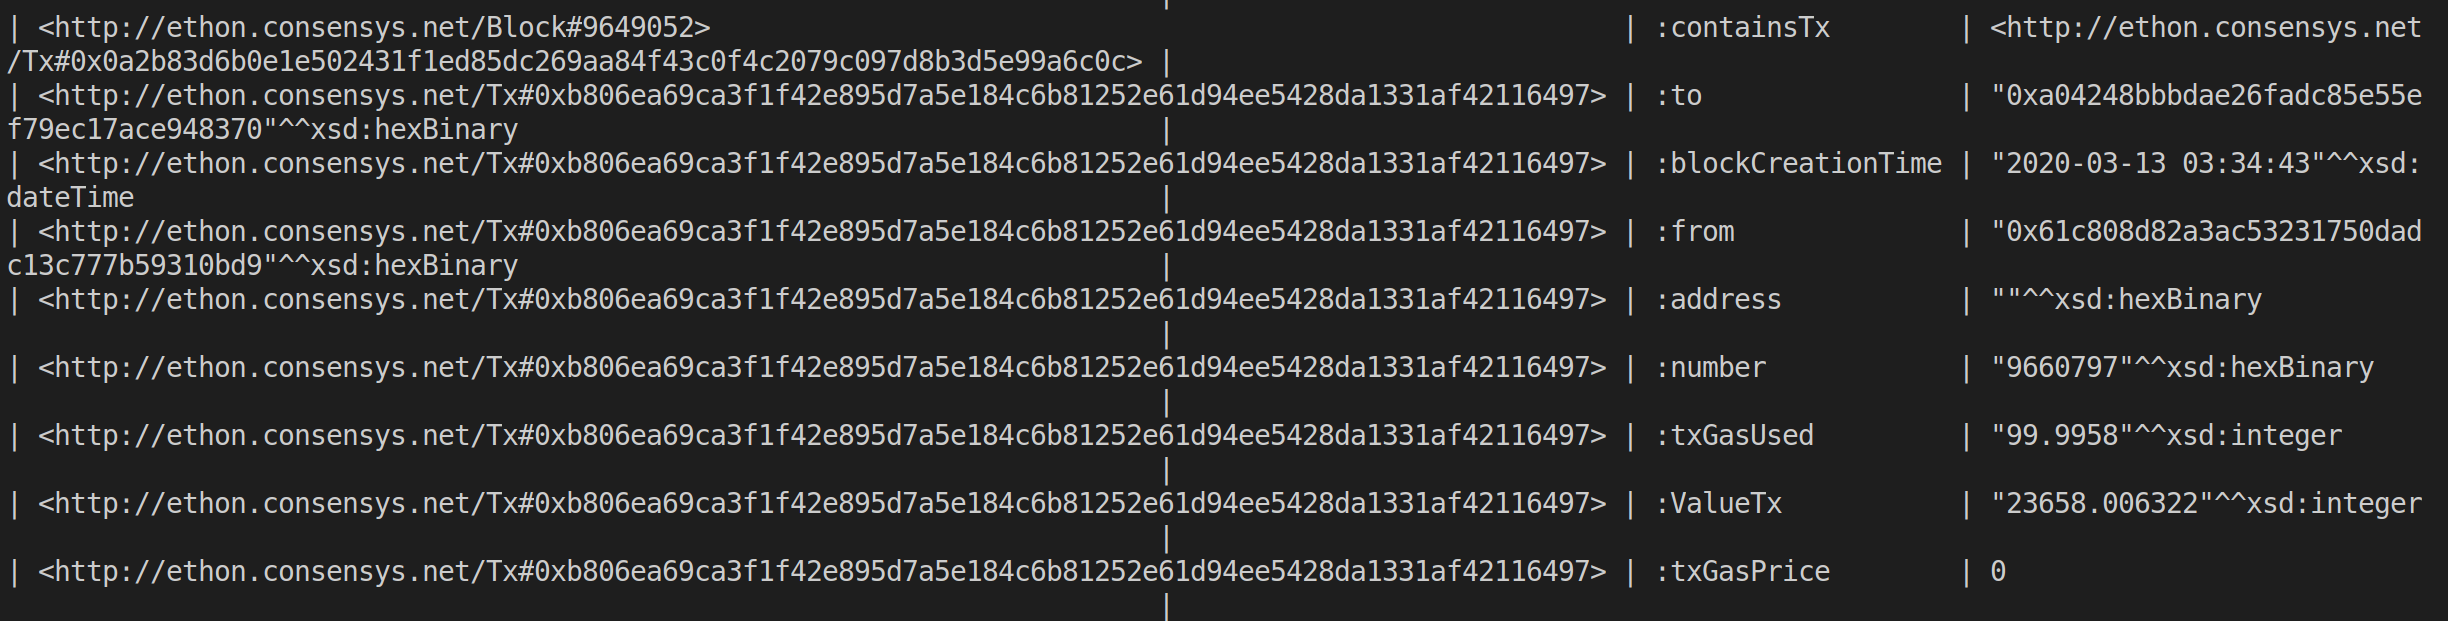
\includegraphics[width=1.55\textwidth]{images/chap03_output_final.png}
		\end{minipage}
		\caption{Final output of a transaction based on SPQRL query}
		
	\end{figure}
	
\end{center}
